\documentclass[12pt]{article} % A4 paper and 11pt font size

\usepackage{lipsum}

\usepackage{style}

\begin{document}

\begin{titlepage}
  \centering
  \Large

  \CreateTitle{Número de práctica}{Título de la práctica}

  \vfill

  \CreateAuthor{Autor}{Correo}

  \vfill

  Grado\\
  Universidad\\
  Asignatura\\
  Curso académico
\end{titlepage}


\tableofcontents

\listoffigures

\listoftables

\pagebreak

%-------------------------------------------------------------------------------
%-------------------------------------------------------------------------------

\section{Presentación del problema}

Example Cite\cite{sample-cite}. Sample fig ref (\autoref{fig:cat1}) and table (\autoref{tab:meas-knn}).

\lipsum[1]

\begin{figure}[H]
    \centering
    \begin{subfigure}[t]{0.49\linewidth}
      \centering
      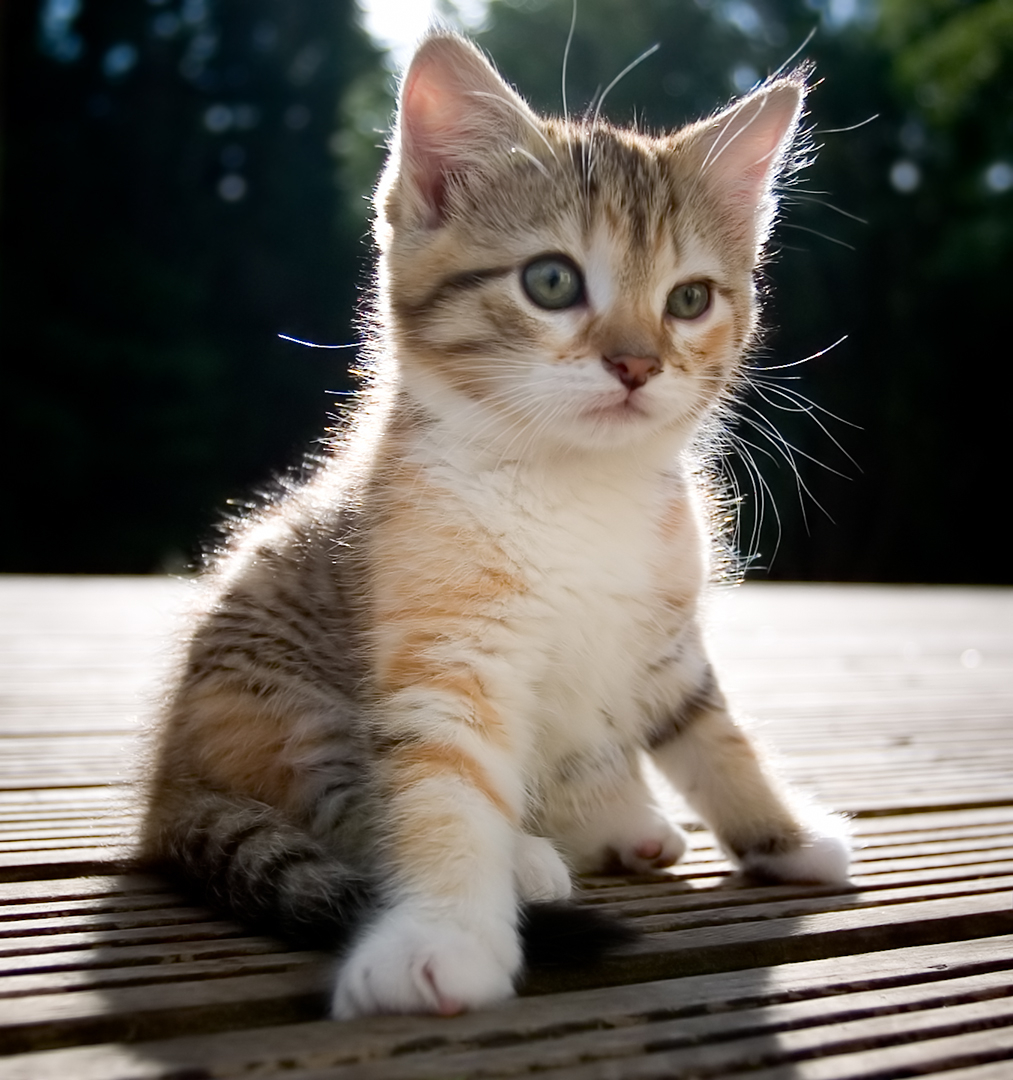
\includegraphics[width=0.8\textwidth]{cat3}
      \caption{A Cat.}
      \label{fig:cat1}
    \end{subfigure}
    \hfill
    \begin{subfigure}[t]{0.49\linewidth}
      \centering
      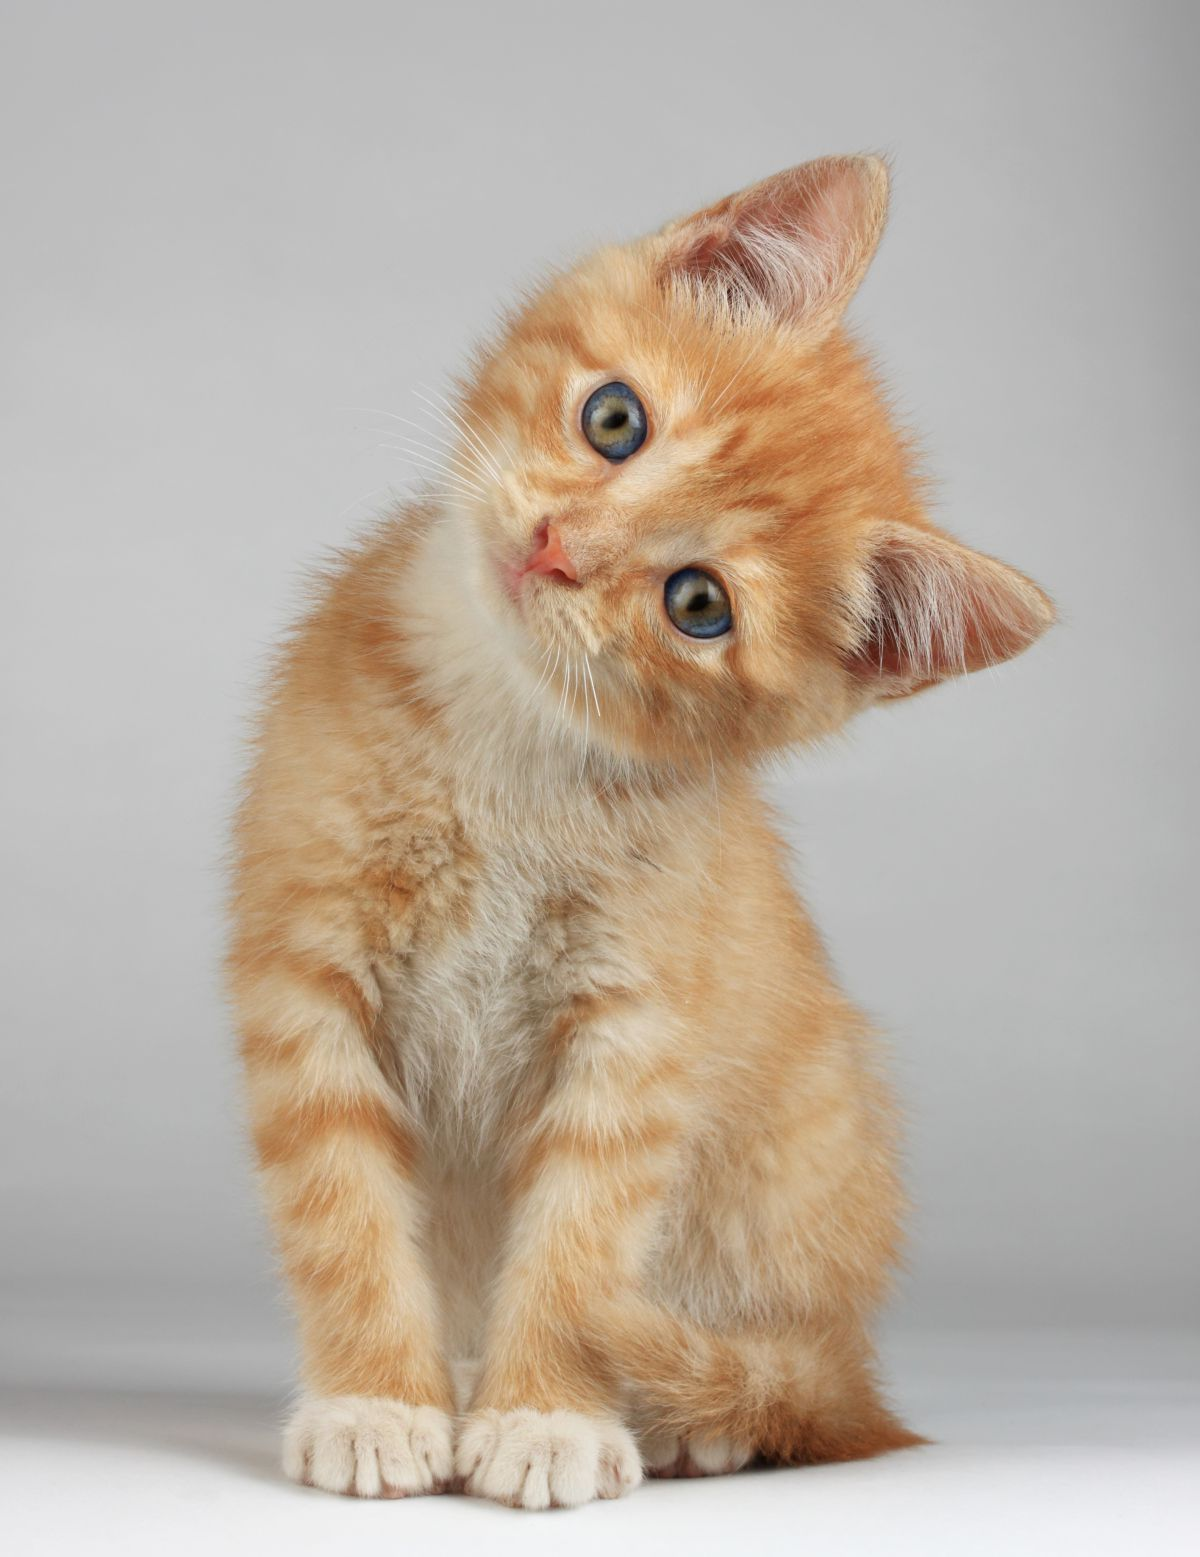
\includegraphics[width=0.8\textwidth]{cat2}
      \caption{Another cat.}
      \label{fig:cat2}
    \end{subfigure}
    \vspace{-5pt}
    \caption{Cats :D}
    \vspace{-25pt}
\end{figure}

\lipsum[2-3]

\begin{wrapfigure}{r}{0.4\textwidth}
  \vspace{-10pt}
  \centering
  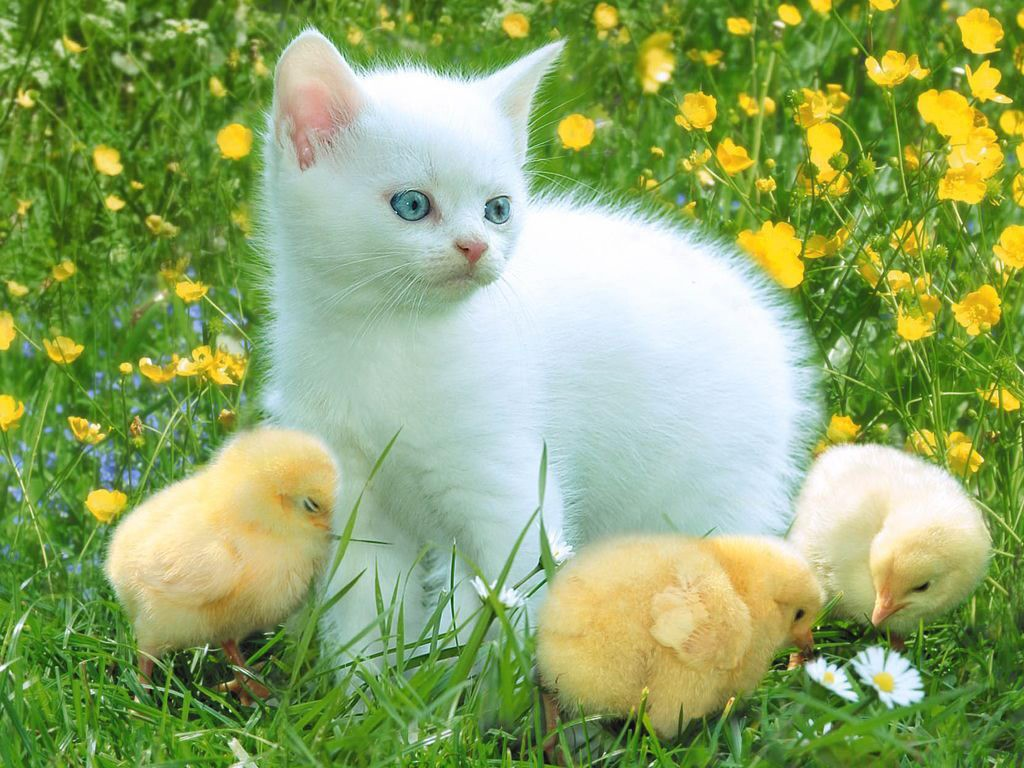
\includegraphics[width=0.35\textwidth]{cat1}
  \caption{A cat}
  \vspace{-20pt}
\end{wrapfigure}

\lipsum[5-7]

%-------------------------------------------------------------------------------

\section{Pruebas realizadas}

\lipsum[8-9]

\begin{figure}[H]
  \centering
  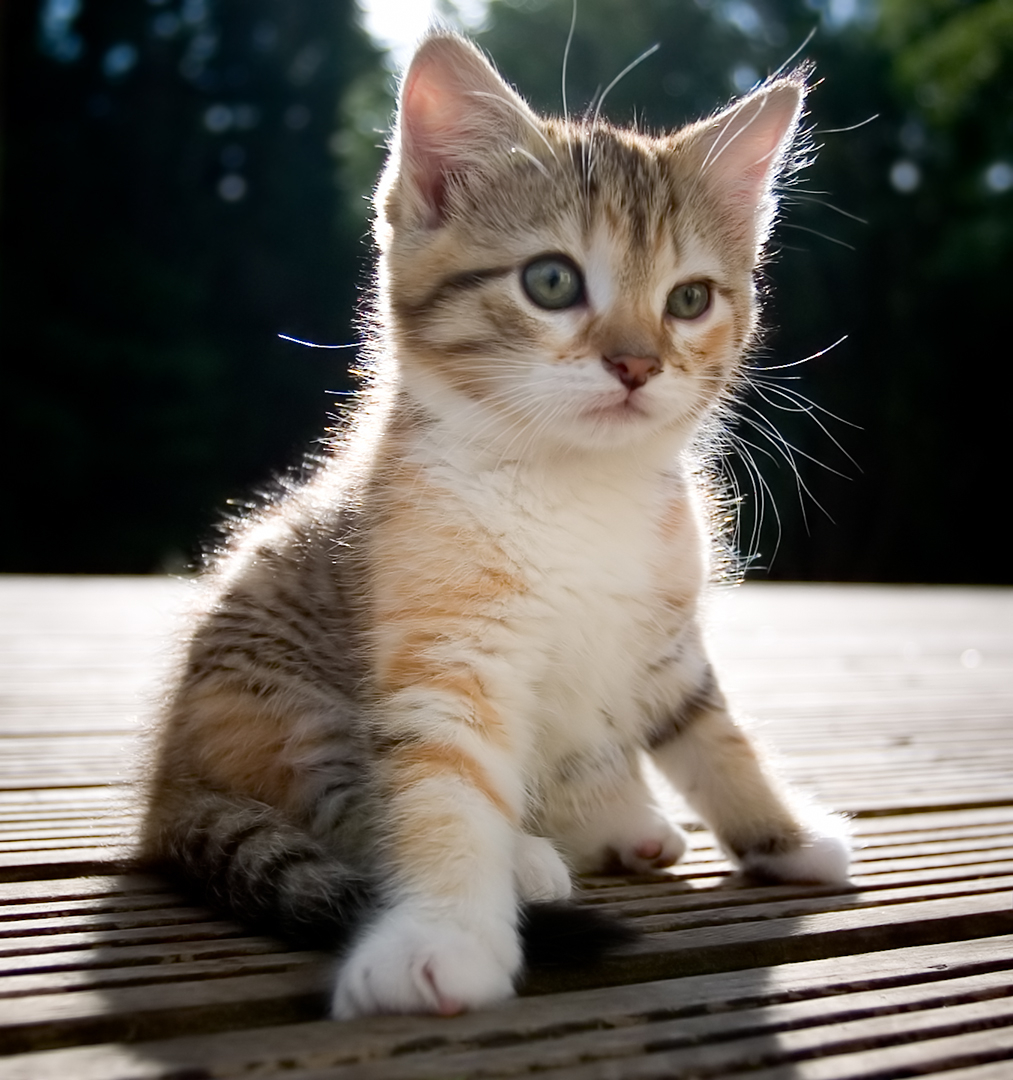
\includegraphics[width=.4\textwidth]{cat3}
  \caption{A Cat.}
  \label{fig:cat3}
  \vspace{-20pt}
\end{figure}

\lipsum[10]

%-------------------------------------------------------------------------------

\section{Resultados obtenidos}

\lipsum[11]

\begin{table}[H]
  \centering
  \begin{tabular}{l | c | c | c | c | c | c}
    & \textbf{Accuracy} & \textbf{TPR} & \textbf{TNR} & \textbf{AUC} & \textbf{F1-Score} & \textbf{G-mean} \\ \hline
    \textit{KNN} & 0.72542 & 0.18466 & 0.88146 & 0.537 & 0.23148 & 0.40345 \\
  \end{tabular}
  \caption{Tabla de resultados de K Nearest Neighbor.}\label{tab:meas-knn}
  \vspace{-20pt}
\end{table}

\lipsum[12]

\subsection{Algoritmo}

\lipsum[13-14]

Algoritmo \autoref{psc:euclid}.

\begin{algorithm}[H]
  \caption{Euclid’s algorithm}\label{psc:euclid}
  \begin{algorithmic}[1]
    \Procedure{Euclid}{$a,b$}\Comment{The g.c.d. of a and b}
    \State $r\gets a\bmod b$
    \While{$r\not=0$}\Comment{We have the answer if r is 0}
    \State $a\gets b$
    \State $b\gets r$
    \State $r\gets a\bmod b$
    \EndWhile\label{euclidendwhile}
    \State \textbf{return} $b$\Comment{The gcd is b}
  \EndProcedure
  \end{algorithmic}
\end{algorithm}

\lipsum[14]

%-------------------------------------------------------------------------------
%-------------------------------------------------------------------------------

\newpage

\bibliography{references} %archivo citas.bib que contiene las entradas
\bibliographystyle{ieeetr} % hay varias formas de citar

\end{document}
